
% this file is called up by thesis.tex
% content in this file will be fed into the main document

%: ----------------------- introduction file header -----------------------
% the code below specifies where the figures are stored
\graphicspath{{2/figures/}}

\chapter{Context}
\label{chp:context}


It goes without saying that we live in the Age of Information, our day to day experiences awash in a flood of data.
We buy, sell, consume and produce information in unprecedented quantities, with countless applications lying at the intersection of our physical world and the virtual one of computers. 
As a result, a variety of specialized disciplines have formed under the auspices of Artificial Intelligence (AI) and information processing, with the intention of developing machines to help us navigate and ultimately make sense of this data.
Coalescing around the turn of the century, music informatics is one such discipline, drawing from several diverse fields including electrical engineering, music psychology, computer science, machine learning, and music theory, among others.
Now encompassing a wide spectrum of application areas and the kinds of data considered---from audio and text to album covers and online social interactions---music informatics can be broadly defined as the study of information related to, or is a result of, musical activity.


From its inception, many fundamental challenges in content-based music informatics, and more specifically those that focus on music audio signals, have received a considerable and sustained research effort from the community. 
This area of study falls under the umbrella of perceptual AI, operating on the premise that if a human expert can experience some musical event from an audio signal, it should be possible to make a machine respond similarly.
As the field continues into its second decade, there are a growing number of resources that comprehensively review the state of the art in these music signal processing systems across a variety of different application areas  \cite{Klapuri2006,Casey2008,Mueller2011a}, including melody extraction, chord recognition, beat tracking, tempo estimation, instrument identification, music similarity, genre classification, and mood prediction, to name only a handful of the most prominent topics.

After years of diligent effort however, there are two uncomfortable truths facing content-based MIR.
First, progress in many well-worn research areas is decelerating, if not altogether stalled.
A review of recent MIREX\footnote{Music Information Retrieval Evaluation eXchange (MIREX): {http://www.music-ir.org/mirex/}} results provides some quantitative evidence to the fact, as shown in Figure \ref{fig:mirex}.
The three most consistently evaluated tasks for more than the past half decade ---chord recognition, genre recognition, and mood estimation--- are each converging to performance plateaus below satisfactory levels.
Fitting an intentionally generous logarithmic model to the progress in chord recognition, for example, estimates that continued performance at this rate would eclipse 90\% in a little over a decade, and 95\% some twenty years after that; note that even this trajectory is quite unlikely, and for only this one specific problem (and dataset).
Attempts to extrapolate similar projections for the other two tasks are even less encouraging.
Second, these ceilings are pervasive across many open problems in the discipline.
Though single-best accuracy over time is shown for these three specific tasks, other MIREX tasks exhibit similar, albeit more sparsely sampled, trends.
Other research has additionally demonstrated that when state-of-the-art algorithms are employed in more realistic situations, i.e. larger datasets, performance degrades substantially \cite{BertinMahieux2012}.
Consequently, these observations have encouraged some to question the state of affairs in content-based MIR:
Does content \emph{really} matter, especially when human-provided information about the content has proven to be more fruitful than the content itself \cite{Slaney2011}? 
If so, what can we learn by analyzing recent approaches to content-based analysis \cite{Flexer2012}? 
Are we considering all possible solutions \cite{Humphrey2012a}? 

\begin{figure}
\begin{centering}
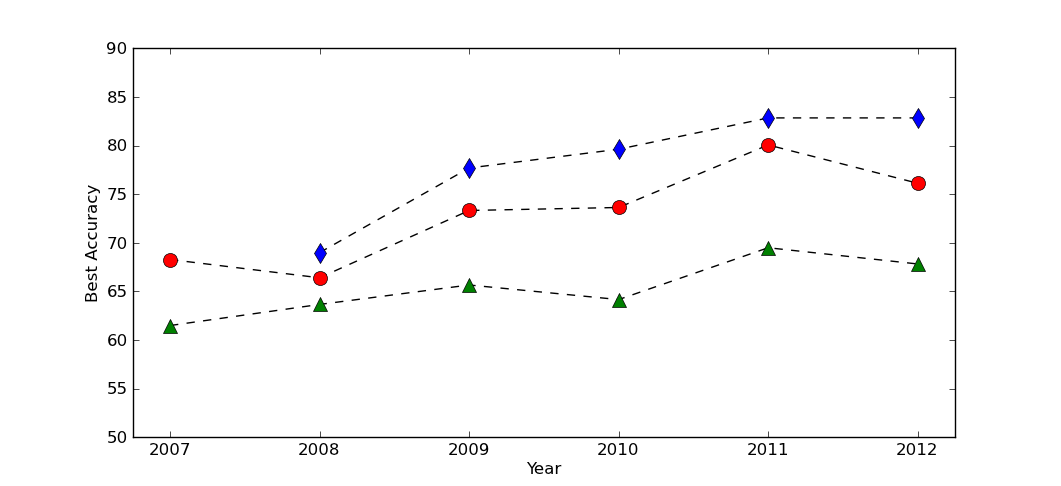
\includegraphics[height=1.5 in]{mirex2}
\caption{\emph{Losing steam}: The best performing systems at MIREX since 2007 are plotted as a function of time for Chord Recognition (blue diamonds), Genre Recognition (red circles), and Mood Estimation (green triangles).}
\label{fig:mirex}
\end{centering}
\end{figure}


The first question directly challenges the raison d'\^etre of computer audition: is content-based analysis still a worthwhile venture?
While applications such as playlist generation \cite{McFee2012} or similarity \cite{Levy2009} have recently seen better performance by using contextual information and metadata rather than audio alone, this approach cannot reasonably be extended to most content-based applications.
It is necessary to note that human-powered systems leverage information that arises as a by-product of individuals listening to and organizing music in their day to day lives.
Like the semantic web, music tracks are treated as self-contained documents that are related to each other through common associations.
However, humans do not naturally provide the information necessary to solve many worthwhile research challenges simply as a result of \emph{passive} listening.
First, listener data are typically stationary over the entire musical document, whereas musical information of interest will often have a temporal dimension not captured at the track-level.
Second, many tasks ---polyphonic transcription or chord recognition, for example--- inherently require an expert level of skill to perform well, precluding most listeners from even intentionally providing this information.

Some may contend that if this information cannot be harvested from crowd-sourced music listening, then perhaps it could be achieved by brute force annotation.
Recent history has sufficiently demonstrated, however, that such an approach simply cannot scale.
As evidence of this limitation, consider the large-scale commercial effort currently undertaken by the Music Genome Project (MGP), whose goal is the widespread manual annotation of popular music by expert listeners.
At the time of writing, the MGP is nearing some 1M professionally annotated songs, at an average rate of 20--30 minutes per track.
By comparison, iTunes now offers over 28M tracks; importantly, this is only representative of commercial music and audio, and neglects the entirety of amateur content, home recordings, sound effects, samples, and so on, which will only make this task more insurmountable. 
Given the sheer impossibility for humans to meaningfully describe all recorded music, truly scalable MIR systems will require good computational algorithms.

Therefore, acknowledging that content-based MIR is indeed valuable, we turn our attention to the other two concerns: what can we learn from past experience, and are we fully exploring the space of possible solutions? 
The rest of this paper is an attempt to answer those questions. 
Section \ref{sec:common} critically reviews conventional approaches to content-based analysis and identifies three major deficiencies of current systems: the sub-optimality of hand-designing features, the limitations of shallow architectures, and the short temporal scope of signal analysis. 
In Section \ref{sec:deeplearning} we contend that \emph{deep learning} specifically addresses these issues, and thus alleviates some of the existing barriers to advancing the field. 
We offer conceptual arguments for the advantages of both \emph{learning} and \emph{depth}, formally define these processing structures, and show how they can be seen as generalizations of current methods. 
Furthermore, we provide specific arguments as to why it is timely for the MIR community to adopt these techniques \emph{now}. 
To further strengthen the latter point, Section \ref{sec:examples} discusses three recent case studies in music informatics that showcase the benefits of deep learning. 
Finally, in Section \ref{sec:future}, we conclude with a survey of challenges and future directions to encourage a more concerted exploration of this promising research topic.


\section{Reassessing Common Practice in Content-based MIR}
\label{sec:common}

Despite a broad spectrum of application-specific problems, the vast majority of music signal processing systems adopt a common two-stage paradigm of feature extraction and semantic interpretation.
Leveraging substantial domain knowledge and a deep understanding of digital signal theory, researchers carefully architect signal processing systems to capture useful signal-level attributes, referred to as \emph{features}.
These statistics are then provided to a pattern recognition machine for the purposes of assigning semantic meaning to observations.
Crafting good features is a particularly challenging subproblem, and it is becoming standard practice amongst researchers to use precomputed features\footnote{Million Song Dataset} or off-the-shelf implementations\footnote{MIR Toolbox, Chroma Toolbox, MARSYAS, Echonest API}, focusing instead on increasingly more powerful pattern recognition machines to improve upon prior work. 
Therefore, while early research mainly employed simple classification strategies such as nearest-neighbors or peak-picking, recent work makes extensive use of sophisticated and versatile techniques, e.g. Support Vector Machines \cite{Mandel2005}, Bayesian Networks \cite{Mauch2010a}, Conditional Random Fields \cite{Sumi2012}, and Variable-Length Markov Models \cite{Chordia2011}.

\begin{figure}
\begin{centering}
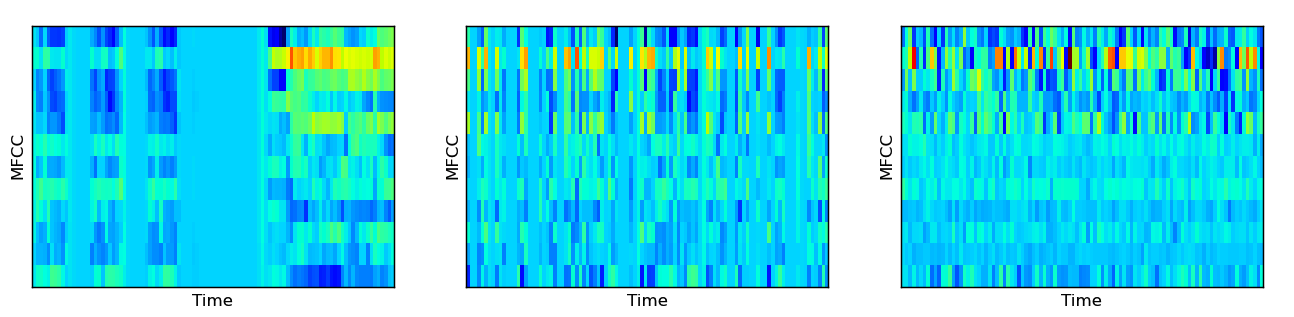
\includegraphics[width=4.5 in]{mtb_mfccs}
\caption{\emph{What story do your features tell?} Sequences of MFCCs are shown for a real music excerpt (left), a time-shuffled version of the same sequence (middle), and an arbitrarily generated sequence of the same shape (right). All three representations have equal mean and variance along the time axis, and could therefore be modeled by the exact same distribution.}
\label{fig:mfccs}
\end{centering}
\end{figure}

This trend of squeezing every bit of information from a stock feature representation is arguably suspect because the two-tier perspective hinges on the premise that \emph{features are fundamental}. 
Data must be summarized in such a way that the degrees of freedom are informative for a particular task; features are said to be \emph{robust} when this is achieved, and \emph{noisy} when variance is misleading or uninformative.
The more robust a feature representation is, the simpler a pattern recognition machine needs to be, and vice versa.
It can be said that robust features \emph{generalize} by yielding accurate predictions of new data, while noisy features can lead to the opposite behavior, known as \emph{over-fitting} \cite{Bishop2006}.
The substantial emphasis traditionally placed on feature design demonstrates that the community implicitly agrees, but it is a point worth illustrating.
Consider the scenario presented in Figure \ref{fig:mfccs}.
The predominant approach to compute how similar two music signals sound is to model their Mel-Frequency Cepstral Coefficients (MFCCs) with a Gaussian Mixture Model (GMM) and compute some distance measure between them, e.g. KL-divergence, Earth mover's distance, etc. \cite{Berenzweig2004}.
Importantly though, representing these coefficients as a mixture of Gaussians reduces the observation to mean and variance statistics, discarding temporal structure.
Therefore, the three MFCC sequences shown ---a real excerpt, a shuffled version of it, and a randomly generated one--- are identical in the eyes of the model.
The audio that actually corresponds to these respective representations, however, will certainly not \emph{sound} similar to a human listener.

This bears a significant consequence: any ambiguity introduced or irrelevant variance left behind in the process of computing features must instead be overcome by the pattern recognition machine.
Previous research in chord recognition has explicitly shown that better features allow for simpler classifiers \cite{Cho2011}, and intuitively many have spent years steadily improving their respective feature extraction implementations \cite{Lyon2010,Mueller2011b}.
Moreover, there is ample evidence these various classification strategies work quite well on myriad problems and datasets \cite{Bishop2006}.
Therefore, underperforming content-based MIR systems are more likely the result of deficiencies in the feature representation than the classifier used to make sense of it. 


It is particularly prudent then, to examine the assumptions and design decisions incorporated into feature extraction systems.
In music signal processing, audio feature extraction typically consists of a recombination of a small set of operations, as depicted in Figure \ref{fig:simplearch}: splitting the signal into independent short-time segments, referred to as blocks or frames; applying an affine transformation, generally interpreted as either a projection or filterbank; applying a non-linear function; and pooling across frequency or time.
Some of these operations can be, and often are, repeated in the process.
For example, MFCCs are computed by filtering a signal segment at multiple frequencies on a Mel-scale (affine transform), taking the logarithm (non-linearity), and applying the Discrete Cosine Transform (affine transformation).
Similarly, chroma features are produced by applying a constant-Q filterbank (affine transformation), taking the complex modulus of the coefficients (non-linearity), and summing across octaves (pooling).

\begin{figure}
\begin{centering}
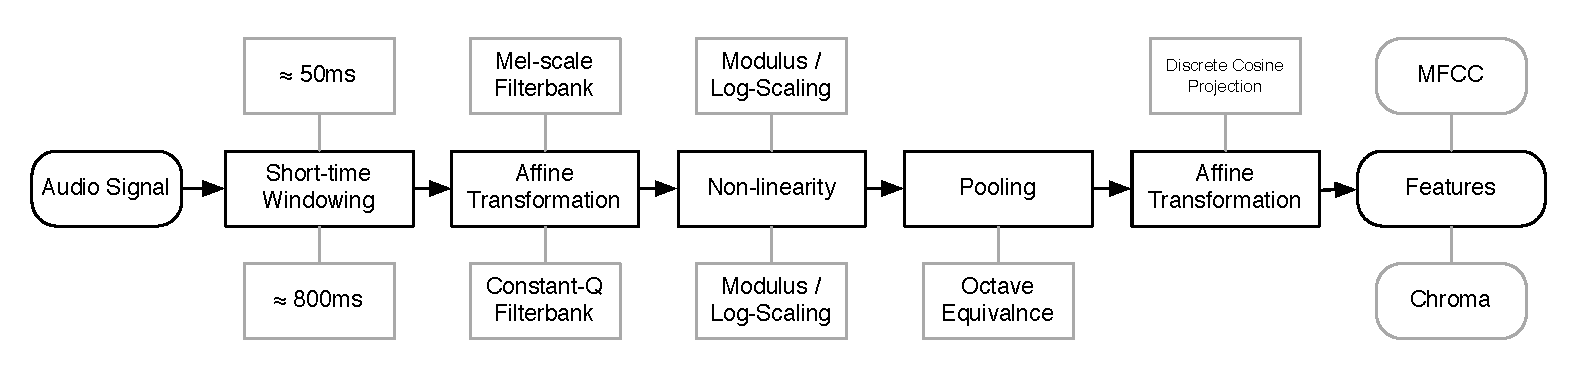
\includegraphics[width=4.75 in]{simplearch}
\caption{\emph{State of the art}: Standard approaches to feature extraction proceed as the cascaded combination of a few simpler operations; on closer inspection, the main difference between chroma and MFCCs is the parameters used.}
\label{fig:simplearch}
\end{centering}
\end{figure}


Considering this formulation, there are three specific reasons why this approach might be problematic. 
First, though the data-driven training of classifiers and other pattern recognition machines has been standard for over a decade in music informatics, the parametrization of feature extractors ---e.g. choice of filters, non-linearities and pooling strategies, and the order in which they are applied--- remains, by and large, a manual process.
Both feature extraction and classifier training present the same basic problem: there is a large solution space and, somewhere in it, a configuration that optimizes an objective function over a dataset.
Though the music informatics community is privileged with a handful of talented researchers who are particularly adept at exploring this daunting space, crafting good features can be a time consuming and non-trivial task.
Additionally, carefully tuning features for one specific application offers no guarantees about relevance or versatility in another scenario.
As a result, features developed for one task ---chroma for chord recognition \cite{Fujishima1999} or MFCCs in speech \cite{Mermelstein1980}--- are used in others they were not specifically designed for, e.g. structural segmentation \cite{Levy2007} or music classification \cite{Mandel2005}. 
The caveat of repurposing features designed for other applications is that, despite potentially giving encouraging results, they are not optimized for this new use case.
In fact, recent research has demonstrated that better features than MFCCs exist for \emph{speech recognition} \cite{Hinton2012}, the very task they were designed for, so it is almost certain that there are better musical features as well.
Therefore, the conclusions to draw from this are twofold: continuing to manually optimize a feature representation is not scalable to every problem, and we may be unnecessarily constraining our search of the solution space.


Second, these information processing architectures can be said to be \emph{shallow}, i.e. incorporating only a few non-linear transformations in their processing chain.
Sound, like other real-world phenomena, naturally lives on a highly non-linear manifold within its time-domain representation.
Shallow processing structures are placed under a great deal of pressure to accurately characterize the latent complexity of this data.
Feature extraction can thusly be conceptualized as a function that maps inputs to outputs with an order determined by its \emph{depth}; for a comprehensive discussion on the merits and mathematics of depth, we refer the curious reader to \cite{Bengio2009}. 
Consider the example in Figure \ref{fig:curvefit}, where the goal is to compute a low-dimensional feature vector (16 coefficients) that describes the log-magnitude spectrum of a windowed violin signal.
One possible solution to this problem is to use a \emph{channel vocoder} which, simply put, low-pass filters and decimates the spectrum, producing a piece-wise linear approximation of the envelope.
It is clear, however, that with only a few linear components we cannot accurately model the latent complexity of the data, obtaining instead a coarse approximation.
Alternatively, the \emph{cepstrum} method transforms the log-magnitude spectrum before low-pass filtering.
In this case, the increase in depth allows the same number of coefficients to more accurately represent the envelope. 
Obviously, powerful pattern recognition machines can be used in an effort to compensate for the deficiencies of a feature representation.
However, shallow, low-order functions are fundamentally limited in the kinds of behavior they can characterize, and this is problematic when the complexity of the data greatly exceeds the complexity of the model.

\begin{figure}[t]
\begin{centering}
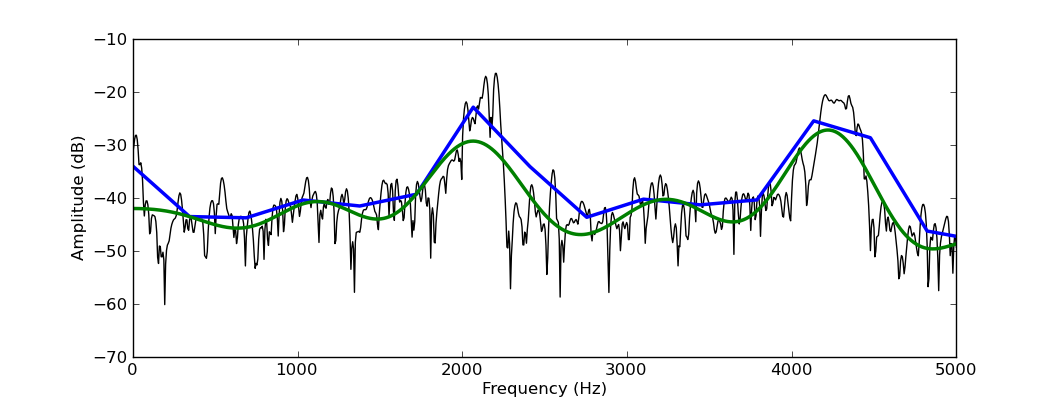
\includegraphics[height=1.5 in]{specfit}
\caption{\emph{Low-order approximations of highly non-linear data}: The log-magnitude spectra of a violin signal (black) is characterized by a channel vocoder (blue) and cepstrum coefficients (green). The latter, being a higher-order function, is able to more accurately describe the contour with the same number of coefficients.}
\label{fig:curvefit}
\end{centering}
\end{figure}

Third, short-time signal analysis is intuitively problematic because the vast majority of our musical experiences do not live in hundred millisecond intervals, but at least on the order of seconds or minutes.
Conventionally, features derived from short-time signals are limited to the information content contained within each segment.
As a result, if some musical event does not occur within the span of an observation ---a motif that does not fit within a single frame--- then it simply cannot be described by that feature vector alone.
This is clearly an obstacle to capturing high-level information that unfolds over longer durations, noting that time is extremely, if not fundamentally, important to how music is perceived.
Admittedly, it is not immediately obvious how to incorporate longer, or even multiple, time scales into a feature representation, with previous efforts often taking one of a few simple forms.
\emph{Shingling} is one such approach, where a consecutive series of features is concatenated into a single, high-dimensional vector \cite{Casey2008}.
In practice, shingling can be fragile to even slight translations that may arise from tempo or pitch modulations.
Alternatively, \emph{bag-of-frames (BoF)} models consider patches of features, fitting the observations to a probability distribution.
As addressed earlier with Figure \ref{fig:mfccs}, bagging features discards temporal structure, such that any permutation of the feature sequence yields the same distribution.
The most straightforward technique is to ignore longer time scales at the feature level altogether, relying on post-filtering \emph{after} classification to produce more musically plausible results.
For this to be effective though, the musical object of interest must live at the time-scale of the feature vector or it cannot truly be encoded.
Ultimately, none of these approaches are well suited to characterizing structure over musically meaningful time-scales.


\subsection{A Concise Summary of Current Obstacles} 
\label{sec:obstacles}
In an effort to understand why progress in content-based music informatics is plateauing, we have reviewed the standard approach to music signal processing and feature design, deconstructing assumptions and motivations behind various decisions. 
As a result, three potential areas of improvement are identified.
So that each may be addressed in turn, it is useful to succinctly restate the main points of this section:

\begin{itemize}

\item \textbf{Hand-crafted feature design is neither scalable nor sustainable}: Framing feature design as a search in a solution space, the goal is to discover the configuration that optimizes an objective function. Even conceding that some gifted researchers might be able to achieve this on their own, they are too few and the process too time-consuming to realistically solve every feature design challenge that will arise. \\
\item \textbf{Shallow processing architectures struggle to describe the latent complexity of real-world phenomena}: Feature extraction is similar in principle to compactly approximating functions. Real data, however, lives on a highly non-linear manifold and shallow, low-order functions have difficulty describing this information accurately. \\
\item \textbf{Short-time analysis cannot naturally capture higher level information}: Despite the importance of long-term structure in music, features are predominantly derived from short-time segments. These statistics cannot capture information beyond the scope of its observation, and common approaches to characterizing longer time scales are ill-suited to music.\\

\end{itemize}

